\lab{Python}{Computer Caches}{Caches}
\objective{Understand the role caches play in computational performance.}

The real computational bottleneck of computers lies in the memory system, not the processor.  
In the early days of computing, memory speed and CPU speed were evenly matched.  
The CPU relatively quickly access data directly from RAM.  
Now, the CPU spends a large amount of time waiting for data to process.  
RAM simply isn't fast enough to keep up.  With CPUs crunching numbers at faster and faster rates, higher performance memory needed to be placed between a relatively slow RAM to cache data.  


\section*{Cache Hits and Cache Misses}
A \emph{cache hit} is where the bytes we request are already in cache.  We avoid having to fall through the different cache levels searching for the data that we want.  When the data we request is not in cache, it is called a \emph{cache miss}.  
Cache misses are performance killers.  Ideally we want to keep relevant data in cache as long a possible before sending it out again.

\section*{Cache lines}
When data is fetched from caches, it fetches bytes that are around the requested byte.  
If we want to access bytes near the initially requested byte it results in a cache hit.
Requested other values in the same cache line has close to no overhead.
The moment we request a byte outside the cache line, we have to search the cache for it.  If it is not in cache, we have a cache miss.
Bytes are brought into the cache in blocks called \emph{cache lines}.
We can measure the cache line size by stepping through an array with different step sizes.
We have done this in Figure \ref{fig:linesize}.  We are using 32 bit integer arrays in all of our tests.
We start to see a drop in run times after a step size of 16.
Since a 32 bit integer is 4 bytes, we arrive at a cache line size of 64 bytes ($4 \mbox{~bytes} * 16 \mbox{~integers} = 64 \mbox{~bytes}$).

\begin{figure}
\centering
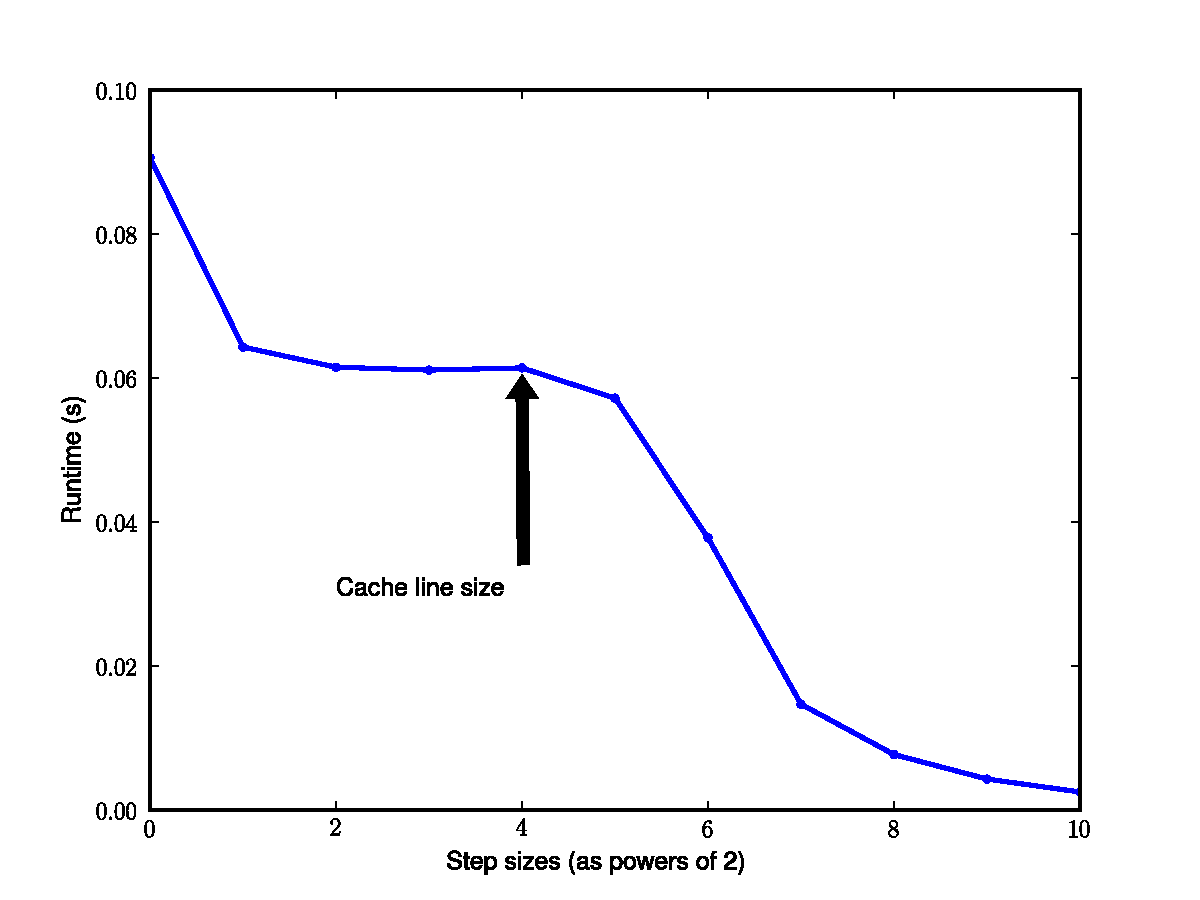
\includegraphics[width=\textwidth]{cache_line.pdf}
\caption{Determining cache line size by looping through a 128MB array with different step sizes.}
\label{fig:linesize}
\end{figure}


\begin{problem}
Find the cache line size for your machine.
To compile you the included C program, you will need a C compiler.
We recommend gcc with the flags \texttt{-O3 -mtune=native}.
The C program expects two arguments: first, the candidate cache line size, and second, the number of loops to run during testing.
The program will print out how many seconds on average one loop took to execute in seconds.
Plot the results of your timings.
\label{prob:cacheline}
\end{problem}

\section*{Cache Size}
Various levels of caches were inserted between main memory and the CPU.  
Level 1 (L1) cache was wired directly into the processor.  Level 2 (L2) cache was wired directly into the motherboard.  
Many multi-core processors these days have a third (L3) cache in addition to L1 and L2 caches.  
L1 cache is smallest cache at around 32 kilobytes with the fastest with access times of around 1 nanosecond.  
L2 cache comes in at about 3 nanoseconds.  L3, the largest, but slowest of the caches, clocks in at about 10 to 20 nanoseconds. 
Main memory finally takes about 100 nanoseconds to access.  L2 caches are typically a few hundred kilobytes for modern processors. 
L3 cache, if present, is generally the largest of the caches with sizes ranging between 1 to 20 megabytes. 
RAM is typically several gigabytes.  If your processor has multiple cores, each core usually has its own separate L1 and L2 caches and share an L3 cache with other other cores.

We can measure the drops in performance that occur when we overflow the cache (Figure \ref{fig:cachesizes}).
We performed measurements on an Intel i7-2640M processor.  The cache line size is 64 bytes

\begin{figure}
\centering
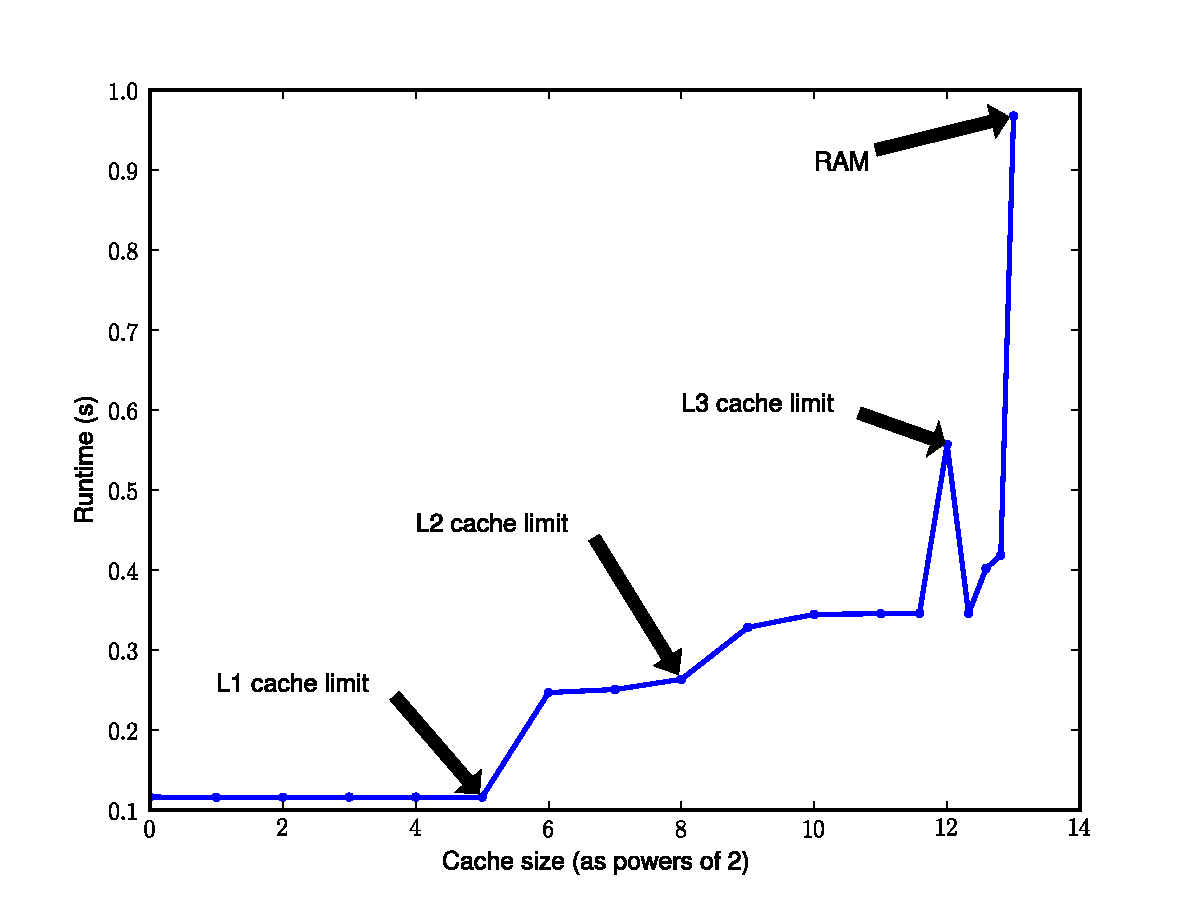
\includegraphics[width=\textwidth]{cache_size.pdf}
\caption{The increases in runtime occur at 32KB, 256KB and 4MB which correspond to the sizes of L1, L2, and L3 caches.}
\label{fig:cachesizes}
\end{figure}


\begin{problem}
Measure the size of your L1 and L2 caches using the cache line value obtained in
Problem \ref{prob:cacheline}.  
To compile you the included C program, you will need a C compiler.
We recommend gcc with the flags \texttt{-O3 -mtune=native}.
The C program expects three arguments: first, the candidate array size, second, the cache line size, and third, the number of loops to run during testing.
The program will print out how many seconds on average one loop took to execute in seconds.
Plot the results of your measurements.
\end{problem}

